\documentclass[a4paper,12pt]{article}
\usepackage[utf8]{inputenc}

\usepackage[utf8]{inputenc}
\usepackage[T2A]{fontenc}
\usepackage[english,russian]{babel}
\usepackage{amsthm}
\usepackage{amsmath}
\usepackage{amssymb}
\usepackage{tikz}
\usepackage{textcomp}
\usepackage{marvosym}
\usepackage{ esint }
\setlength{\topmargin}{-0.5in}
\setlength{\textheight}{9.1in}
\setlength{\oddsidemargin}{-0.4in}
\setlength{\evensidemargin}{-0.4in}
\setlength{\textwidth}{7in}
\setlength{\parindent}{0ex}
\setlength{\parskip}{1ex}
\newcommand{\ndiv}{\hspace{-4pt}\not|\hspace{2pt}}
\usepackage{graphicx}
\usepackage{float}
\usepackage{wrapfig}
\usepackage{pgfplots}
\usepackage{caption}
\pgfplotsset{compat=1.16}
\graphicspath{ {./images/} }
\usepackage{graphicx}
\RequirePackage{caption}
\DeclareCaptionLabelSeparator{defffis}{ — }
\captionsetup{justification=centering,labelsep=defffis}
\usepackage{caption} \captionsetup[table]{labelsep=endash,justification=justified,singlelinecheck=false,font=normalsize}
\usepackage{amsfonts,mathtools}

\title{Лабораторная работа № 3.5.1\\Изучение плазмы газового разряда в неоне}
\author{Илья Прамский}
\date{Ноябрь 2023}

\begin{document}

\maketitle
\newpage
\section*{Введение}
\begin{flushleft}
  \textbf{Цель работы:} изучение вольт-амперной характеристики тлеющего разряда; изучение свойств плазмы методом зондовых характеристик.
\end{flushleft}

\begin{flushleft}
  \textbf{В работе используются:} стеклянная газоразрядная трубка, наполненная неоном, высоковольтный источник питания, источник питания постоянного тока, делитель напряжения, резистор, потенциометр, амперметры, вольтметры, переключатели.
\end{flushleft}

\textit{Двойным зондом} называется система, состоящая их двух одинаковых зондов, расположенных на небольшом расстоянии друг от друга. Между зондами создаётся разность потенциалов $U$, которая по велиине много меньше плавающего потенциала: $\left|U\right|\ll\left|U_f\right|$. При этом оба зонда имеют относительно плазмы близкий к плавающему отрицательный потенциал, т.е. находятся на \textit{ионной} ветви вольт-амперной характеристики.

При отсутствии разности потенциалов ток между зондами равен нулю. Рассчитаем величину тока, проходящего через двойной зонд вблизи точки $I=0$. При небольших разностях потенциалов ионные токи на оба зонда равны ионному току насыщения и компенсируют друг друга. Величина результирующего тока целиком связана с различием в электронных токах. Пусть потенциал на первом зонде равен\[U_1=U_f+\Delta U_1,\]а на втором\[U_2=U_f+\Delta U_2.\]Предполагается, что $\Delta U_1,\Delta U_2\ll U_f$. Напряжение $U$ между зондами равно\[U=U_2-U_1=\Delta U_2-\Delta U_1.\]

Найдём ток, приходящий на первый электрод:\[I_1=I_{i\text{н}}-I_{e0}\exp{\left(\frac{eU_1}{k_{\text{Б}T_e}}\right)}=I_{i\text{н}}-\left[I_{e0}\exp{\left(\frac{eU_f}{k_{\text{Б}T_e}}\right)}\right]\exp{\left(\frac{e\Delta U_1}{k_{\text{Б}T_e}}\right)}.\]Заметим, что при $\Delta U_1=0$ (при $U_1=U_f$) электронный и ионный ток компенсируют друг друга. Это означает, что заключённый в квадратные скобки множитель равен $I_{i\text{н}}$. Имеем поэтому\[I_1=I_{i\text{н}}\left[1-\exp{\left(\frac{e\Delta U_1}{k_{\text{Б}T_e}}\right)}\right].\]Аналогично для второго электрода\[I_2=I_{i\text{н}}\left[1-\exp{\left(\frac{e\Delta U_2}{k_{\text{Б}T_e}}\right)}\right].\]

Заметим, что зонды 1 и 2 соединены \textit{последовательно} -- через плазму -- поэтому $I_1=-I_2=I$. Выразим $\Delta U_1$ и $\Delta U_2$ из уравнений выше:\[\Delta U_1=\frac{k_{\text{Б}}T_e}{e}\ln{\left(1-\frac{I}{I_{i\text{н}}}\right)},\ \Delta U_2=\frac{k_{\text{Б}}T_e}{e}\ln{\left(1+\frac{I}{I_{i\text{н}}}\right)}.\]Наконец, вычитая второе равенство из первого, найдём\[U=\Delta U_1-\Delta U_2=\frac{k_{\text{Б}}T_e}{e}\ln{\left(\frac{I_{i\text{н}}-I}{I_{i\text{н}}+I}\right)},\]и, разрешая это равенство относительно $I$, получим\[I=I_{i\text{н}}\th{\frac{eU}{2k_{\text{Б}}T_e}}.\]Эту формулу можно использовать для определения температуры электронов по форме вольт-амперной характеристики двойного зонда.

Наблюдаемая на опыте зависимость тока от напряжения изображена на рисунке 1. Заметим, что эта кривая отличается от теоретической существованием наклона у асимптот в области больших $\left|U\right|$, что связано с ускорением частиц плазмы приложенным полем, которое не учтено при выводе теоретической зависимости.

Графики типа 1 проще всего обрабатывать следующим образом. Сначала находится ток насыщения $I_{i\text{н}}$ из пересечения асимптот с осью $U=0$. Затем находится наклон графика в начале координат, из которого можно определить температуру электронов $T_e$. Дифференциируя формулу для $I$ по $U$ в точке $U=0$ и принимая во внимание, что при малых аргументах $\th{x}\approx x$, найдём\[k_{\text{Б}}T_e=\frac{1}{2}\frac{eI_{i\text{н}}}{\frac{\text{d}I}{\text{d}U}\vert{}_{U=0}},\]где $\frac{\text{d}I}{\text{d}U}\vert{}_{U=0}$ -- наклон характеристики зонда вблизи начала координат. По известным $T_e$ и $I_{i\text{н}}$ можно найти концентрацию заряженных частиц $n_i=n_e$.

Таким образом, двойные зонды удобно применять для измерения электронной температуры и концентрации частиц в плазме.

\begin{figure}[h]
	\centering
	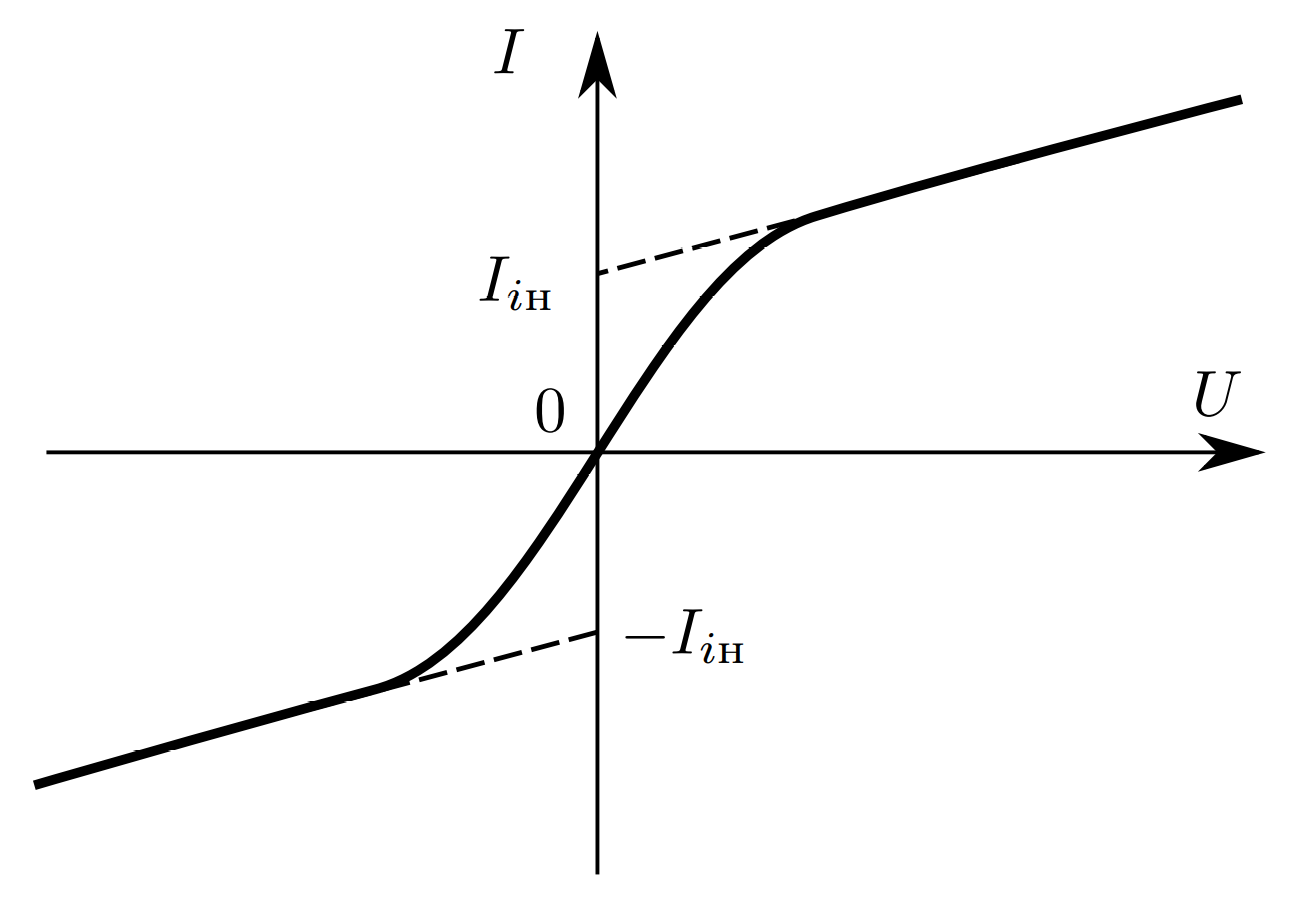
\includegraphics[scale=0.30]{Tok}
	\caption{Вольт-амперная характеристика двойного зонда} \label{Tok}
\end{figure}

\section*{Экспериментальная установка}

Схема установки для исследования плазмы газового разряда в неоне представлена на рисунке 2. Стеклянная газоразрядная трубка имеет холодный (ненагреваемый) полый катод, три анода и \textit{геттерный узел} -- стеклянный балон, на внутреннюю поверхность которого напылена газопоглощающая плёнка (\textit{геттер}). Трубка наполнена изотопом неона ${}^{22}\text{Ne}$ при давлении 2 мм рт. ст. Катод и один из анодов (I или II) с помощью переключателя $\text{П}_1$ подключаются через балластный резистор $R_{\text{б}}$ ($\sim450~\text{к}\Omega$) к регулируемому высоковольтному источнику питания (ВИП) с выходным напряжением до 5 кВ.

\begin{figure}[h]
	\centering
	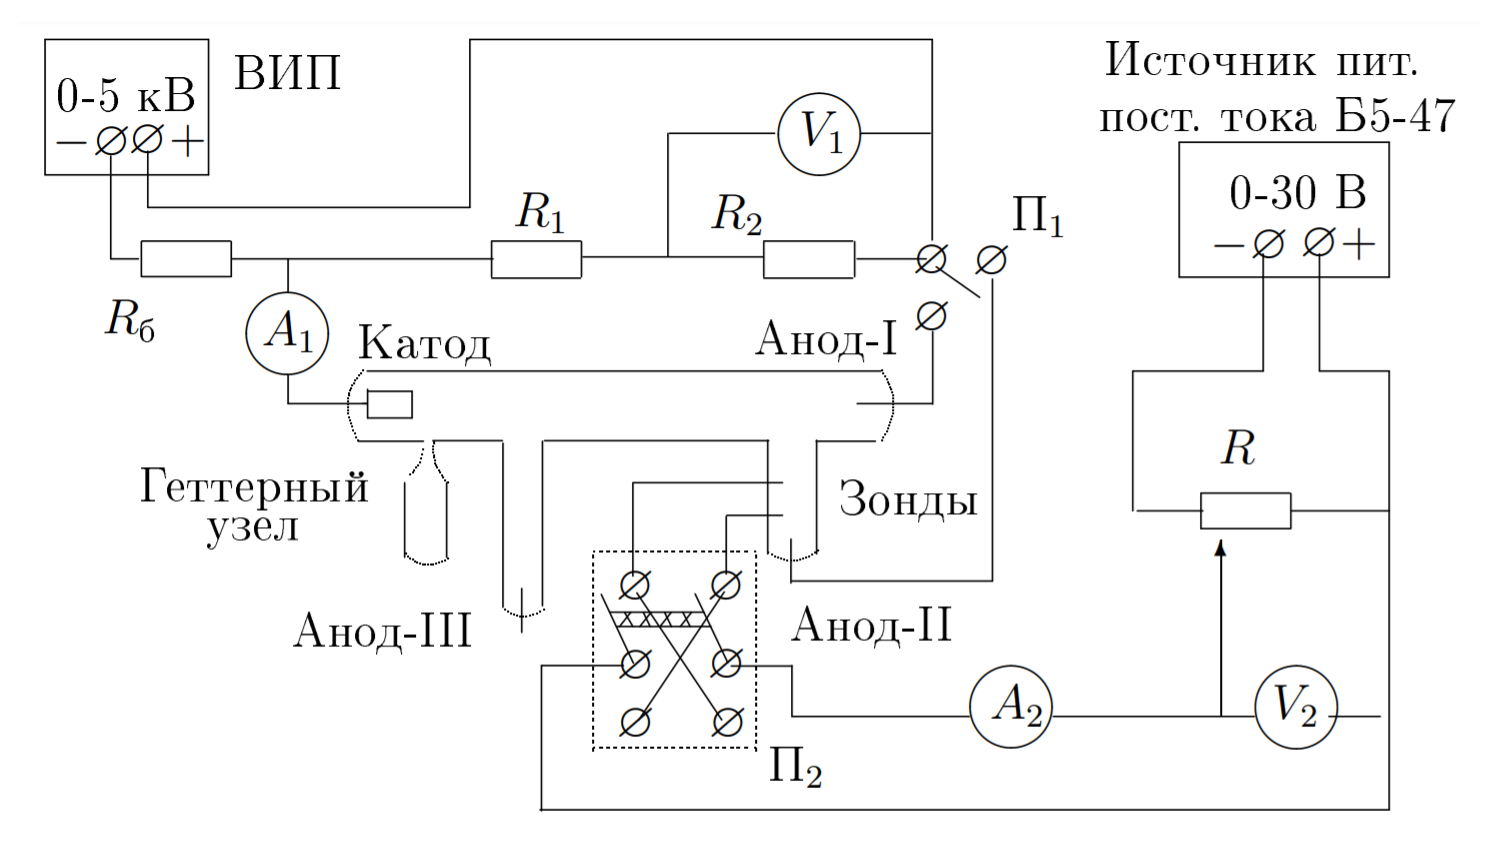
\includegraphics[scale=0.30]{Device}
	\caption{Схема установки для исследования газового разряда} \label{Device}
\end{figure}

При подключении к ВИП анода-I между ним и катодом возникает газовый разряд. Ток разряда измеряется миллиамперметром $A_1$, а падение напряжение на разрядной трубке -- цифровым вольтметром $V_1$ (мультиметром GDM), подключённым к трубке через высоомный ($25~\text{М}\Omega$) делитель напряжения с коэффициентом $\frac{R_1+R_2}{R_2}=10$.

При подключении к ВИП анода-II разряд возникает в пространстве между катодом и анодом-II, где находится двойной зонд, используемый для диагностики плазмы положительного столба.

Зонды изготовлены из молибденовой проволоки диаметром $d=0,2~\text{мм}$ и имеют длину $l=5,2~\text{мм}$. Они подключены к источнику питания GPS через потенциометр $R$. Переключатель $\text{П}_2$ позволяет изменять полярность напряжения на зондах. Величина напряжения на зондах изменяется с помощью дискретного переключателя "$V$" выходного напряжения источника питания и потециометра $R$, а измеряется цифровым вольтметром $V_2$ (GMD). Для измерения зондового тока используется мультиметр $A_2$ (GDM). Анод-III в нашей работе не используется.
\newpage
\section*{Ход работы}
Для начала установим переключатель $\text{П}_1$ в положение \glqq Анод-I\grqq. Затем, плавно увеличивая напряжение ВИП, найдем напряжение зажигания разряда. В нашем случае $U_{\text{заж}} = 193$ В.

Теперь будем менять ток разряда $I_p$ и снимать вольт-амперную характеристику разряда. Данные внесем в таблицу и по ним изобразим график зависимости $I_p(U_p)$.

\begin{figure}[H]
	\begin{center}
    		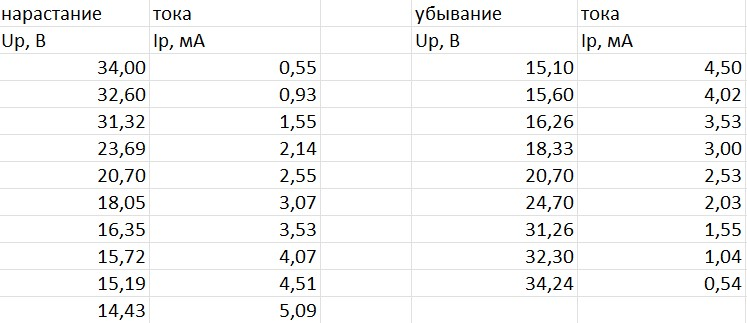
\includegraphics[width=.5\textwidth]{tabliza1.jpg}
    	\end{center}
\end{figure}

\begin{figure}[H]
	\begin{center}    		
    		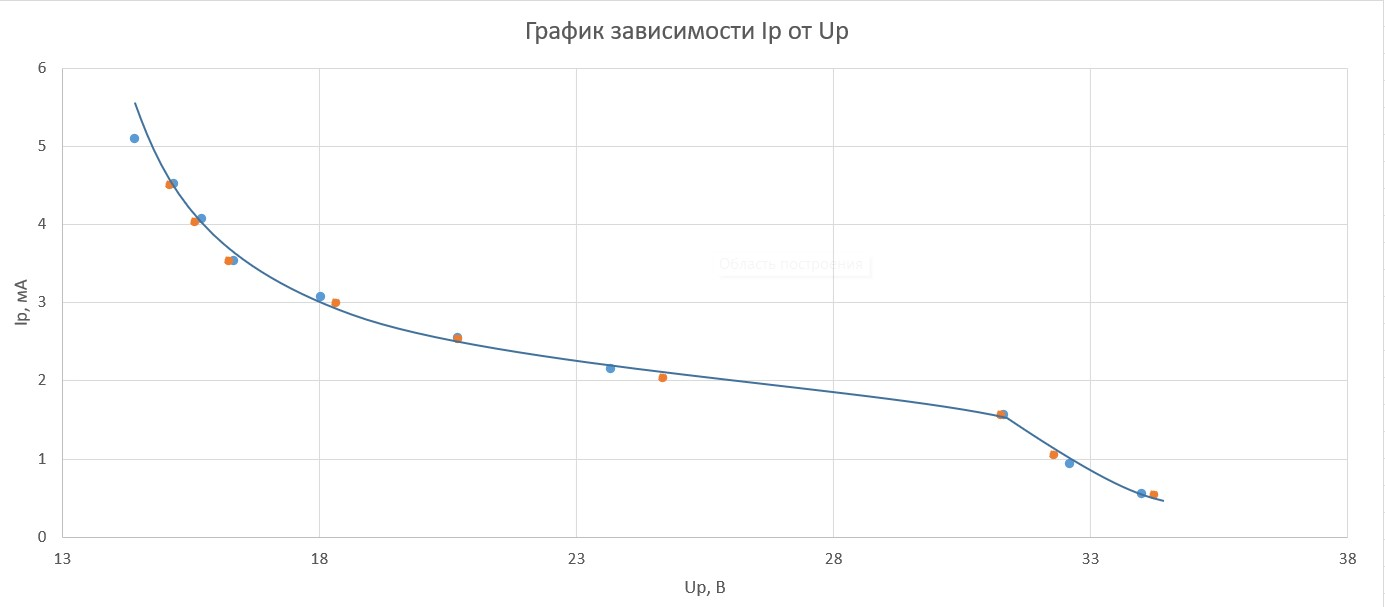
\includegraphics[width=1\textwidth]{graphik1.jpg}
    	\end{center}
\end{figure}

По минимальному наклону кривой, определим максимальное дифференциальное сопротивление разряда $R_{\text{диф}} = \frac{dU}{dI} = -13200$Ом. Также сравним наш участок с графиком из приложения. Легко заметить, что данный участок соответствует участку Г-Д на рисунке из приложения.

\begin{figure}[H]
	\begin{center}    		
    		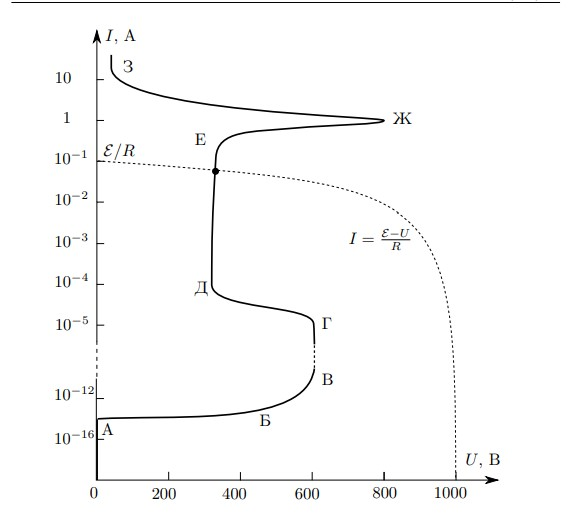
\includegraphics[width=.5\textwidth]{priloshenie.jpg}
    	\end{center}
\end{figure}

Теперь же установим переключатель $\text{П}_1$ в положение \glqq Анод-II\grqq, а переключатель $\text{П}_2$ в положение \glqq +\grqq. Сначала зафиксируем ток разряда(в нашем случае он будет принимать 3 значения: $5,05 ;3,02 ; 1,51$ мА), а затем, установив на зонде максимальное напряжение $U = 25$В, будем снижать его до $U = -25$ В(отрицательные напряжения получаются при изменении положения переключателя 2 на \glqq -\grqq) и фиксировать значения напряжения и тока двойного зонда. По этим данным построим зависимость $I_{\text{з}}(U_{\text{з}})$.

\begin{figure}[H]
	\begin{center}
    		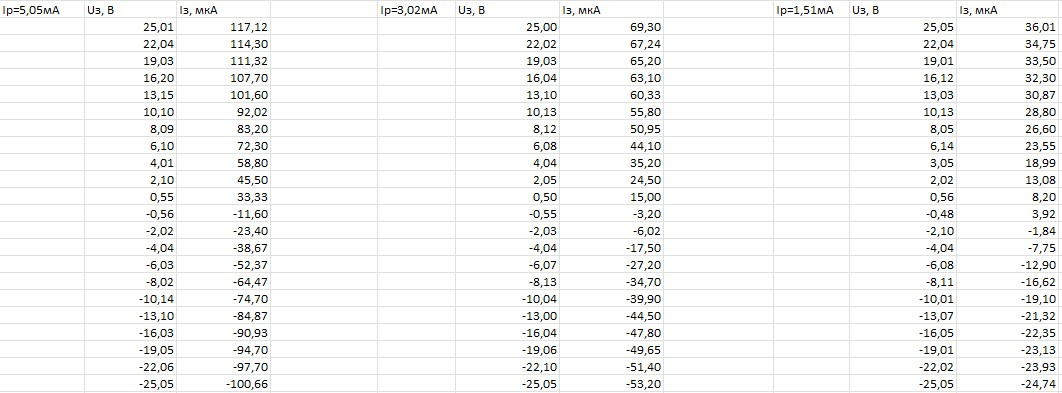
\includegraphics[width =1\textwidth]{tabliza2.jpg}
    	\end{center}
\end{figure} 

\begin{figure}[H]
	\begin{center}    		    		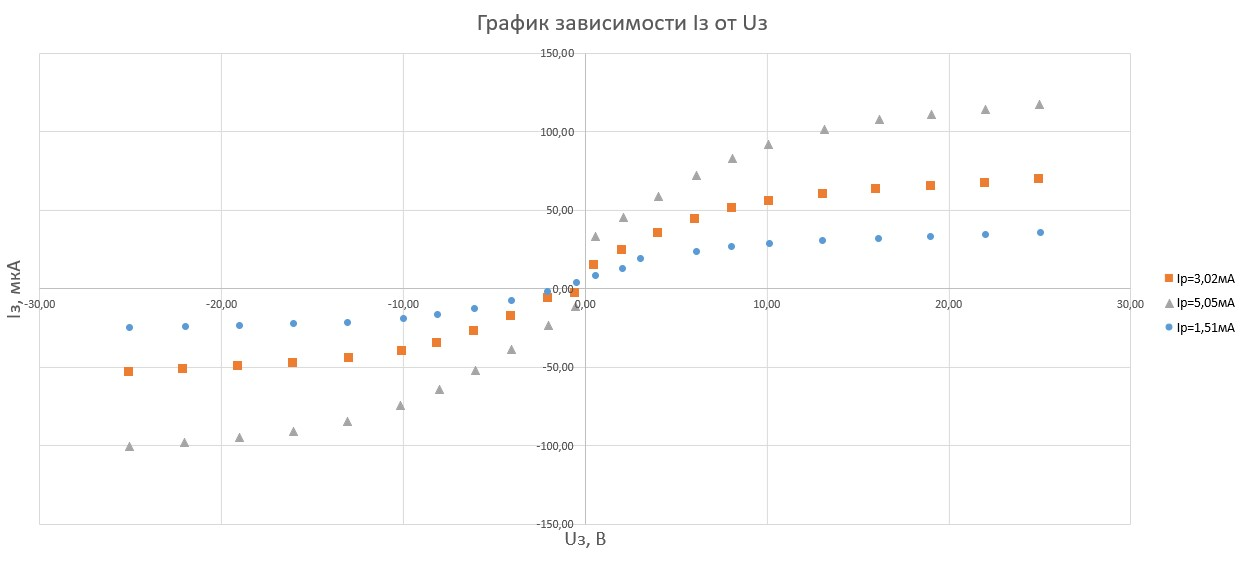
\includegraphics[width=1\textwidth]{graphik5.jpg}
    	\end{center}
\end{figure}

По полученным графикам определим несколько величин. Ток насыщения получим при пересечении асимптоты с осью ординат. $\frac{dI}{dU}|_{u=0}$ найдем из касательной к кривой в нуле. $\Delta U$ определим, как напряжение в точке, полученной пересечением горизонтали при токе равном току насыщения с касательной графика в нуле.

\begin{figure}[H]
	\begin{center}    		
    		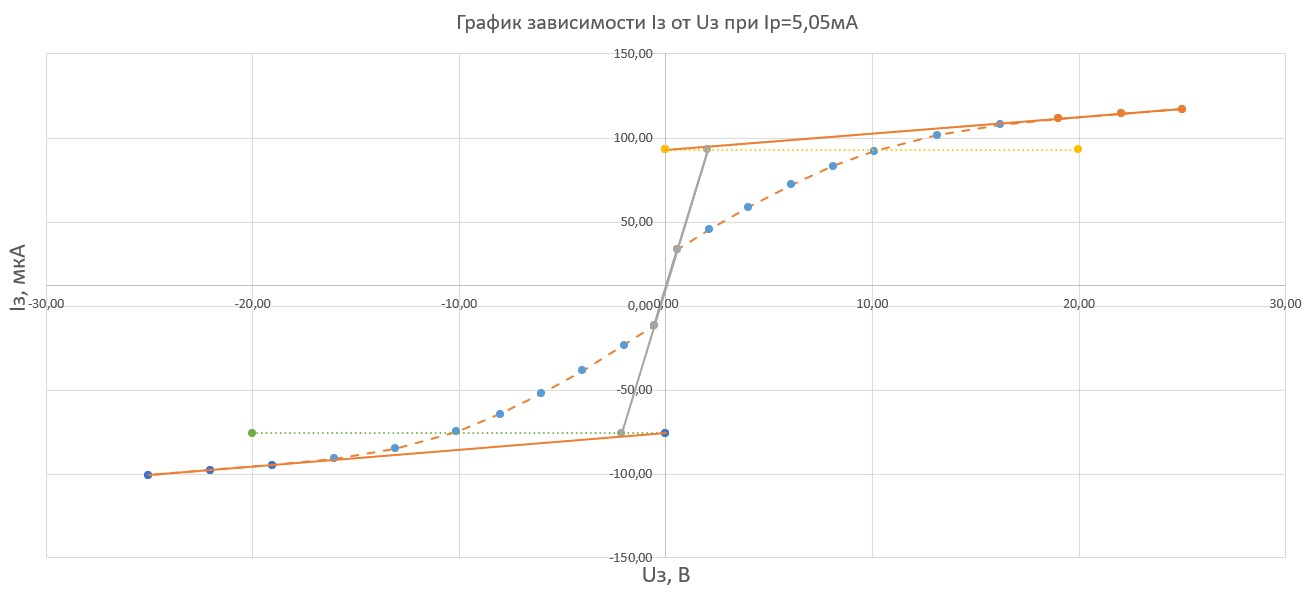
\includegraphics[width=1\textwidth]{graphik2.jpg}
    	\end{center}
\end{figure}

\begin{figure}[H]
	\begin{center}    		
    		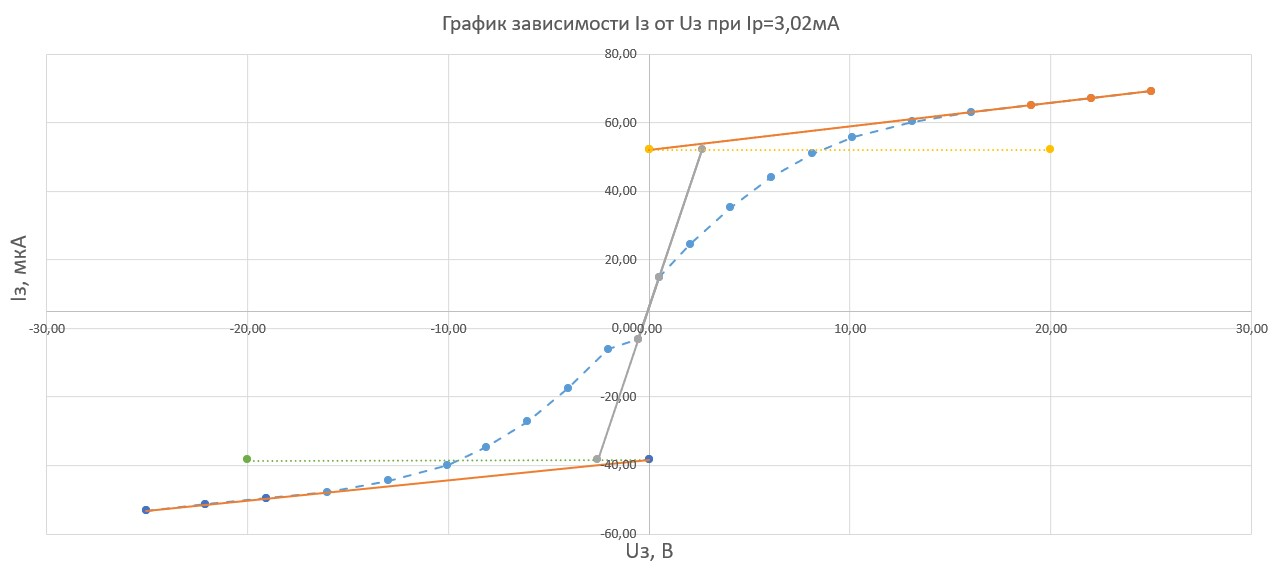
\includegraphics[width=1\textwidth]{graphik3.jpg}
    	\end{center}
\end{figure}

\begin{figure}[H]
	\begin{center}    		
    		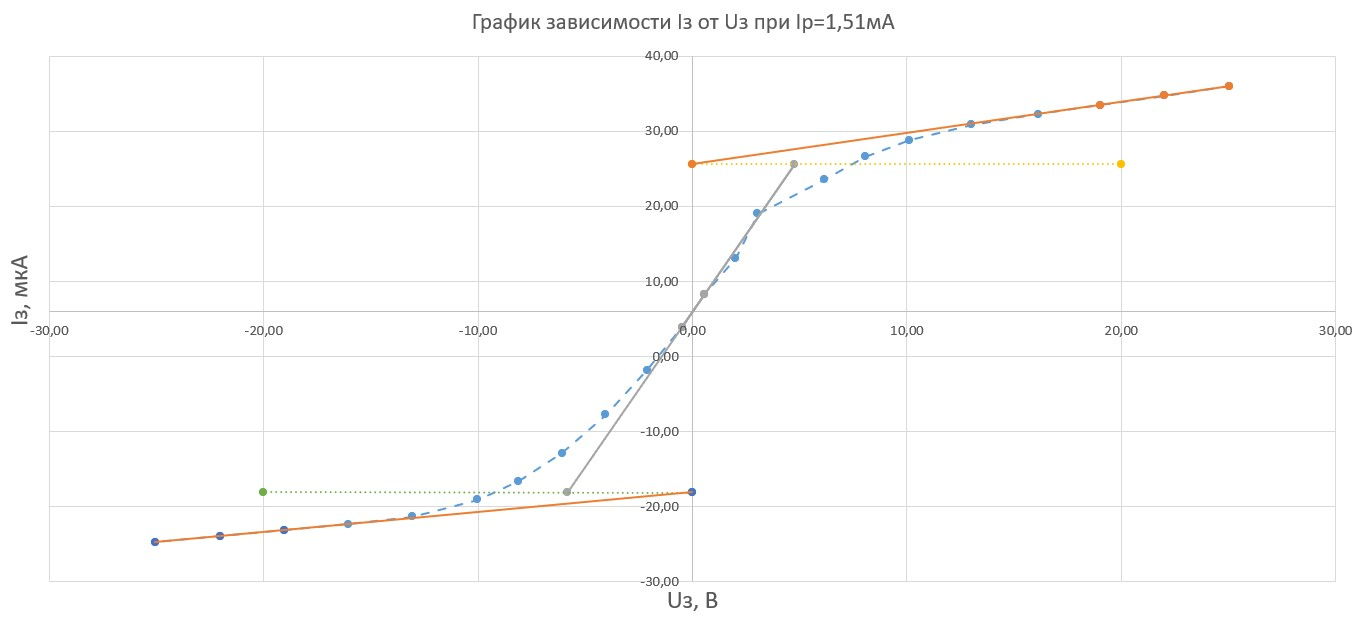
\includegraphics[width=1\textwidth]{graphik4.jpg}
    	\end{center}
\end{figure}
\newpage
Полученные значения приведены в таблице

\begin{figure}[H]
	\begin{center}
    		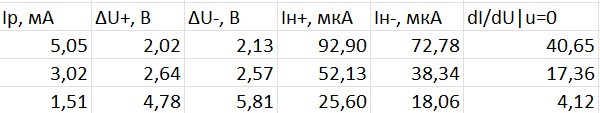
\includegraphics[width =.5\textwidth]{tabliza3.jpg}
    	\end{center}
\end{figure} 

Будем брать значение $\Delta U_+$, т.к. оно более точное(при смене полярности подключения возникали колебания напряжения и тока). Зная $\Delta U$, найдем значение температуры электрона по формуле
\[kT_e = \frac{e \cdot \Delta U}{2} = \frac{\Delta U}{2} \text{эВ}\]
Результаты занесём в итоговую таблицу

Определим концентрацию электронов $n_e$, считая её равной концентрации ионов $n_i$ и используя формулу Бома:\[I_{i\text{н}}=0,4n_eeS\sqrt{\frac{2kT_e}{m_i}}\implies n_e=\frac{2,5I_{i\text{н}}}{eS}\sqrt{\frac{m_i}{2kT_e}}\]где $S=\pi dl$ -- площадь поверхности зонда, а $m_i=22\cdot1,66\cdot10^{-27}~\text{кг}$ -- масса иона неона. Посчитанные по формуле значения $n_e$ тоже занесём в таблицу.

Зная концентрацию электронов в плазме, несложно найти их плазменную частоту колебаний по формуле\[\omega_p=\sqrt{\frac{4\pi n_ee^2}{m_e}}\ \left[\text{СГС}\right]=5,6\cdot10^4\sqrt{n_e}\ \left[\text{СГС}\right]=5,6\cdot10^1\sqrt{n_e}\ \left[\text{СИ}\right].\]Результаты также занесём в таблицу. Заметим, что при падении на эту плазму электромагнитного излучения через неё пройдут волны с частотами, \textit{превышающими} $\omega_p$.

Рассчитаем теперь электронную полряизационную длину $r_{De}$. Используем формулу\[r_{De}=\sqrt{\frac{kT_e}{4\pi n_ee^2}}=\frac{1}{\omega_p}\sqrt{\frac{e\Delta U}{2m_e}}.\]Занесём результаты в таблицу.

По формуле\[r_{D}=\sqrt{\frac{kT_i}{4\pi n_ee^2}}=\frac{1}{\omega_p}\sqrt{\frac{kT_i}{m_e}},\]где $T_i\approx300~\text{К}$, найдём дебаевский радиус. Занесём результаты в таблицу. Из полученных значений ($10^{-4}\ldots10^{-3}~\text{см}$) очевидно, что плазму \textit{можно считать квазинейтральной} при всех используемых в работе токах разряда.

Оценим теперь среднее число ионов $N_D$ в дебаевской сфере:\[N_D=\frac{4\pi}{3}r_D^3n_i.\]Занесём результаты в таблицу. Из полученных значений ($N_D\gg1$) делаем вывод, что \textit{плазма является идеальной}.

Давление в плазме приближённо равно $P\approx2~\text{торр}=266,6~\text{Па}$, тогда можно найти полную концентрацию как $n=\frac{P}{kT_i}=6,44\cdot10^{22}$. Степень ионизации плазмы равна\[\alpha=\frac{n_i}{n},\]посчитанные по этой формуле значения занесём в таблицу.

Также занесём в таблицу дифференциальное сопротивление ВАХ разряда при соответствующих значениях $I_{\text{р}}$.

\begin{figure}[H]
	\begin{center}
    		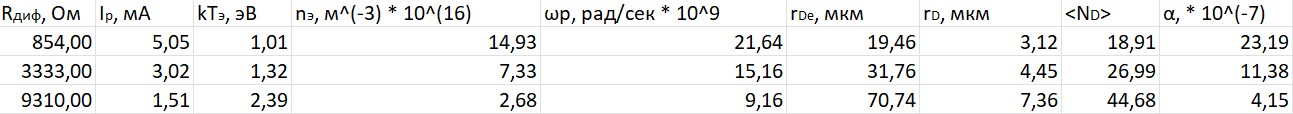
\includegraphics[width =1\textwidth]{tabliza4.jpg}
    	\end{center}
\end{figure} 

Теперь построим графики зависимостей $T_\text{э}(I_p)$ и $n_\text{э}(I_p)$.

\begin{figure}[H]
	\begin{center}
    		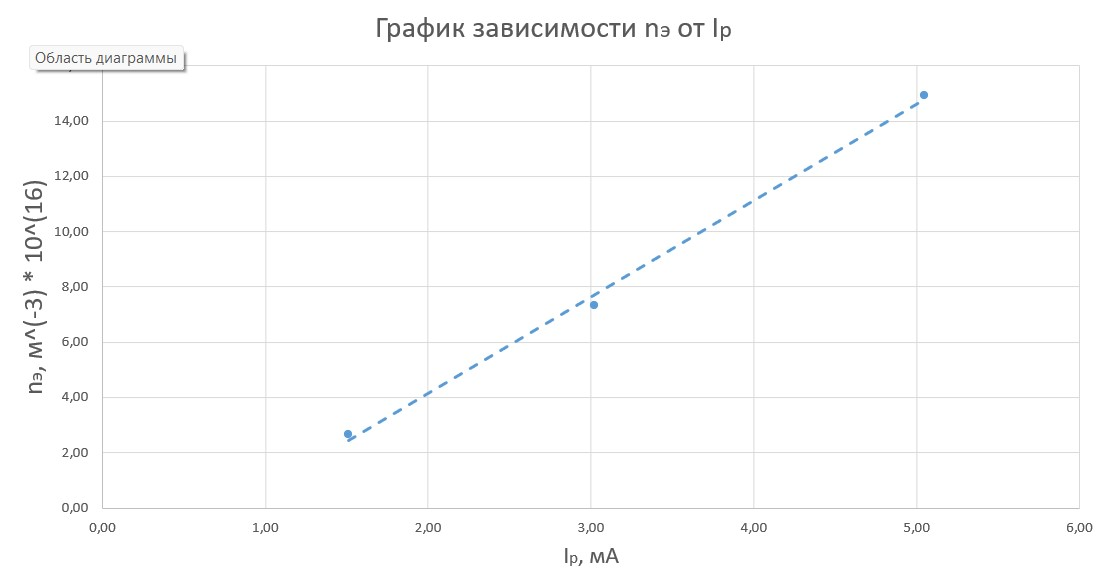
\includegraphics[width =1\textwidth]{graphik6.jpg}
    	\end{center}
\end{figure} 

\begin{figure}[H]
	\begin{center}
    		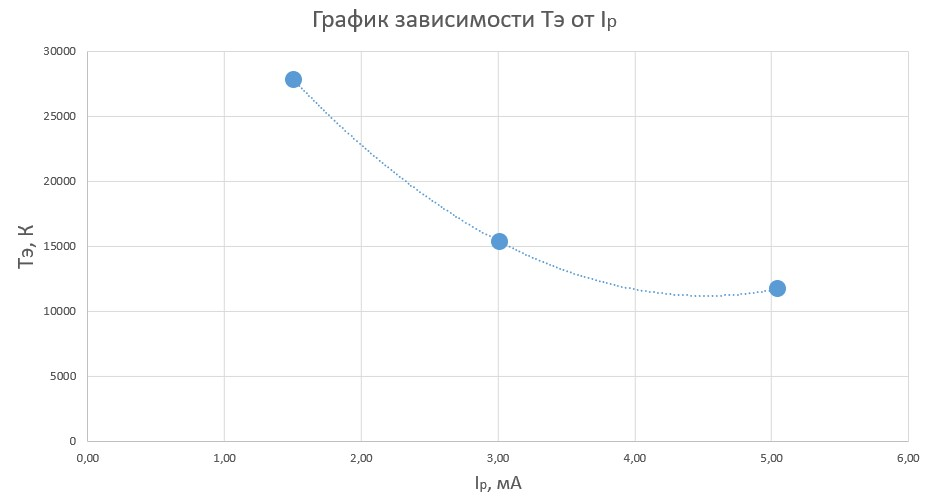
\includegraphics[width =1\textwidth]{graphik7.jpg}
    	\end{center}
\end{figure} 

\section*{Вывод}
В ходе данной работы была изучена вольт-амперная характеристика тлеющего заряда. Также было замечено, что получившийся график является участок истинного графика(Г-Д). Также были изучены свойства плазмы методом зондовых характеристик. Используя двойной зонд, были получены основные характеристики, описывающие плазму, также была исследована зависимость различных величин от тока разряда.
\end{document}
